\documentclass[aps,showpacs,twocolumn,twoside,groupedaddress]{revtex4}
\usepackage{graphicx}
\usepackage{epsfig}
%\usepackage{caption}
%\usepackage{subcaption}
\usepackage{epsf}
\usepackage{amssymb}
\usepackage{epstopdf}
\usepackage{amsmath}
\usepackage{braket}
\usepackage{multirow}
\usepackage{array}
\usepackage{mathrsfs}
\usepackage{bm}
\usepackage{wasysym}
\let\vec\bm

\makeatletter
\renewcommand{\fnum@figure}{Fig. \thefigure}
\makeatother

\begin{document}

\title{The steady state population inversion of $\Xi$-type atoms in the squeezed vacuum reservoir}
\author{Jieyu You, Zeyang Liao, and M. Suhail Zubairy}
\affiliation{Institute for Quantum Science and Engineering (IQSE) and Department of Physics and Astronomy, Texas A$\&$M University, College Station, TX 77843-4242, USA }

\begin{abstract}
We study the steady state of $\Xi$-type atoms coupled to the squeezed vacuum reservoir in the quasi-one-dimensional waveguide. We show that the population inversion can occur as the steady state when the coupling strength of two transitions of the $\Xi$-type atom to the squeezed vacuum are properly set. We also discuss the possibility of the population inversion of a group of atoms in the squeezed vacuum. 
\end{abstract}
\pacs{42.30.-d, 42.50.Hz, 42.62.Fi}\maketitle 


\section{Introduction}
The concept of population inversion is of fundamental importance in laser physics because the production of population inversion is a key step in the workings of a standard laser. However, a population inversion can never exist for a system at thermal equilibrium because of the spontaneous emission. To achieve population inversion therefore requires pushing the system into a non-equilibrated state\cite{svelto1998principles}. In 1946, Purcell showed that the spontaneous decay rate of an emitter can be modified by engineering the electromagnetic bath environment with which the emitters interact\cite{purcell1946purcell}. One example of bath engineering is the squeezed vacuum. Although the squeezed vacuum does not change the density of the electromagnetic modes, it can still modify the decay rate of the emitter\cite{gardiner1986cw, collett1984mj,gea1988vacuum}. For two level atoms, The difference between the squeezed vacuum and the thermal reservoir with the same average photon number mainly resides in the dephasing rate\cite{gardiner1987cw, palma1989gm, agarwal1990cooperative, ficek1990spontaneous,ficek1991z, goldstein1996ev}. In addition, the previous calculations mainly consider a broadband squeezing
in all directions of the 3-dimensional (3D) space which is difficult to be experimentally realized. In contrast
to the 3D case, squeezing in 1D is more experimentally feasible. Suppression of the radiative decay of atomic coherence and the linewidth of the resonance fluorescence have been experimentally demonstrated in a 1D microwave transmission line coupled to single artificial atom\cite{turchette1998qa,murch2013kw, toyli2016resonance, bergeal2010analog, wang2018cavity,qin2018exponentially}. 

In our study, we consider the $\Xi$-type atoms coupled to the broadband squeezed vacuum in the quasi-one-dimensional waveguide. and we found that the population of steady state is completely different than that in the thermal reservoir. We also demonstrate that the complete population inversion can be achieved with proper parameters.

\section{Master equation of three level atoms in the squeezed vacuum}
In this section, we consider a scenario where $N_a$ $\Xi$-type atoms are located inside the waveguide with the squeezed vacuum injected from both ends, as shown in Fig.~\ref{1}(a). The atomic electronic structure is shown in Fig.~\ref{1}(b) where the atomic states are labeled $|a\rangle$, $|b\rangle$, $|c\rangle$ from the excited state to the ground state. We assume that $\omega_{ac}=2\omega_0$ where $\omega_0$ is the center frequency of the broad band squeed vacuum.  $\omega_{ab}$ and $\omega_{bc}$ are not equal but they are still within the bandwith of the squeezed vacuum. We assume that the squeezed vacuum bandwidth is much larger than $|\omega_{ab}-\omega_{bc}|$ so it forms a squeezed vacuum reservoir. 
\begin{figure*}
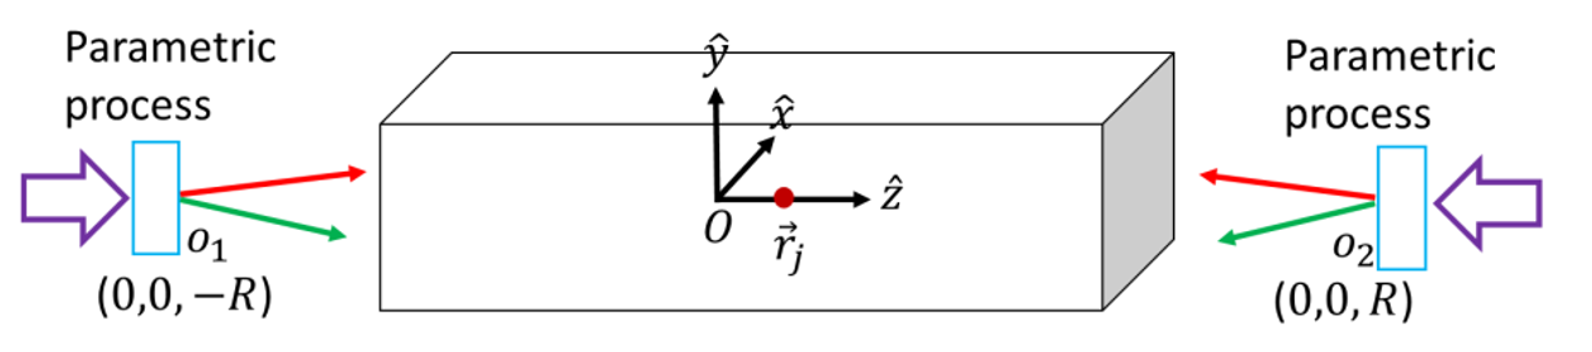
\includegraphics[width=1.5\columnwidth]{fig1.eps}
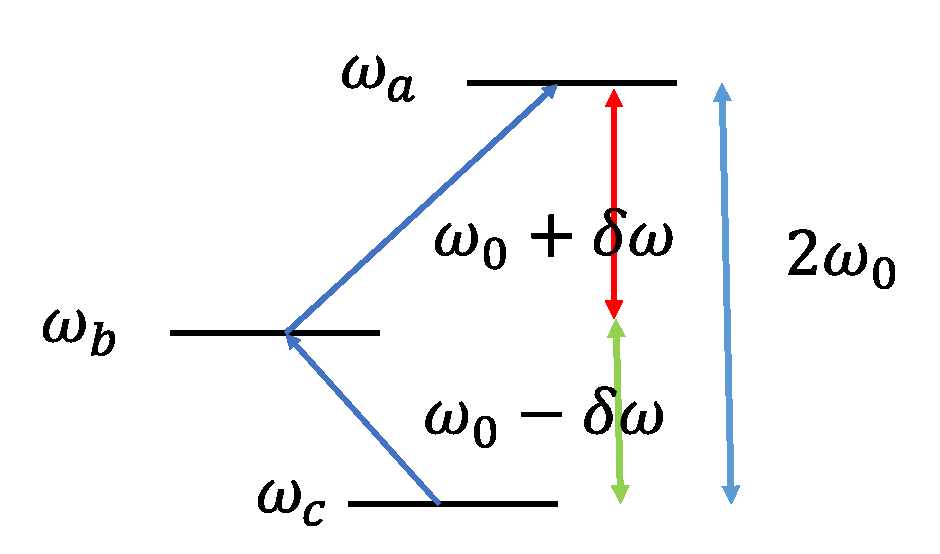
\includegraphics[width=0.5\columnwidth]{fig2.eps}
\caption{(a) Schematic setup: A $\Xi$-type atom is located inside the waveguide with the broadband squeezed vacuum incident from both ends. (b)The energy structure of the three level atom. Transition $|a\rangle\rightarrow|c\rangle$ is forbidden and $\omega_{ac}=2\omega_0$ where $\omega_0$ is the center frequency of the squeezed vacuum. $\omega_{ab}$ and $\omega_{bc}$ differ by a small amount $2\delta\omega_0$ and they are within the bandwidth of the squeezed vacuum reservoir.}
\label{1}
\end{figure*}


%The general master equation of dipole-dipole interaction in the squeezed vacuum can be used to study the dynamics of the three-level atom\cite{You2018}:

The atom-field system is described by the Hamiltonian \begin{equation}
  \label{eq1}
  \begin{gathered}
H=H_{A}+H_{F}+H_{AF}
 \end{gathered}
\end{equation}
where
$H_{A}=\sum_{e=a,b,c}\sum_{l=1}^{N_a}\hbar\omega_{e,l}\left|e_{l}\right\rangle \left\langle e_{l}\right|$  
is the atomic Hamiltonian, and $ \left|e_{l}\right\rangle $ is the energy state of the $l$th atom with energy $\hbar\omega_{e,l}$. The Hamiltonian of the EM field is
$H_{F}=\sum_{\vec{k}s}\hbar\omega_{\vec{k}s}(\hat{a}_{\vec{k}s}^{\dagger}\hat{a}_{\vec{k}s}+\frac{1}{2})$
where $\hat{a}_{\vec{k}s}$ and $\hat{a}_{\vec{k}s}^{\dagger}$ are the annihilation and creation operators of the filed mode with wavevector $ \vec{k}$, polarization $s$, and frequency $\omega_{\vec{k},s}$. The interaction Hamiltonian in electric-dipole approximation is
$H_{AF}=-i\hbar\sum_{\vec{k}s}\sum_{i=1,2}\sum_{l=1}^{N_{a}}[\vec{\mu}_{l,i}\cdot\vec{u}_{\vec{k}s}(\vec{r}_{l,i})S_{l,i}^{+}\hat{a}_{\vec{k}s}+\vec{\mu}_{l,i}^{*}\cdot\vec{u}_{\vec{k}s}(\vec{r}_{l,i})S_{l,i}^{-}\hat{a}_{\vec{k}s}-H.c.]$
where $ \vec{\mu}_{l,i} $ is the electric dipole moment for $ith$ transition of the $l$th atom, where $i=1$ denotes the transition from $|a\rangle$ to $|b\rangle$, and $i=2$ denotes the transition from $|b\rangle$ to $|c\rangle$. $ S_{l,i}^{+} $ and $S_{l,i}^{-} $ are the raising and lowering operator for transition $i$ of the $l$th atom. The mode function of the squeezed vacuum is given by
\begin{equation}
  \label{eq2b}
  \begin{gathered}
\vec{u}_{\vec{k}s}(\vec{r}_{i})=\sqrt{\frac{\omega_{\vec{k}s}}{2\epsilon_{0}\hbar V}}\vec{e}_{ks}e^{i\vec{k}\cdot(\vec{r}_{i}-\vec{o}_{\vec{k}s})}
 \end{gathered}
\end{equation}
where $\vec{o}_{\vec{k}s} $ is a phenomenological parameter which includes the effects of the initial phase and the position of the squeezing source\cite{You2018}. The correlation functions for the squeezed vacuum are\cite{scully1999quantum}:
\begin{equation}
\label{eq0a}
\begin{split}
& \left\langle a_{\vec{k},s}^{\dagger}a_{\vec{k}',s'}\right\rangle =\sinh^{2}r\delta_{\vec{k}'\vec{k}}\delta_{ss'} \\
& \left\langle a_{\vec{k},s}a_{\vec{k}',s'}^{\dagger}\right\rangle =\cosh^{2}r\delta_{\vec{k}'\vec{k}}\delta_{ss'}\\
& \left\langle a_{\vec{k},s}^{\dagger}a_{\vec{k}',s'}^{\dagger}\right\rangle =-e^{-i\theta}\cosh(r)\sinh(r)\delta_{\vec{k}',2\vec{k}_{0}-\vec{k}}\delta_{ss'}\\
&\left\langle a_{\vec{k},s}a_{\vec{k}',s'}\right\rangle =-e^{i\theta}\cosh(r)\sinh(r)\delta_{\vec{k}',2\vec{k}_{0}-\vec{k}}\delta_{ss'}
\end{split}
\end{equation}
For simplicity, we can set the squeezing parameter $\theta=0$, and all atoms to align along the same direction. The dynamics of the atomic system can be described by the following master equation(See Appendix A for details of derivation):
\begin{widetext}
\begin{equation}
\label{eq1}
\begin{split}
\frac{d\rho^{S}}{dt}=&-i\underset{i\neq j}{\sum}\Lambda_{ij}[S_{i}^{+}S_{j}^{-},\rho^{S}]e^{i(\omega_{i}-\omega_{j})t}-\frac{1}{2}\underset{i,j}{\sum}\gamma{}_{ij}(1+N)(\rho^{S}S_{i}^{+}S_{j}^{-}+S_{i}^{+}S_{j}^{-}\rho^{S}-2S_{j}^{-}\rho^{S}S_{i}^{+})e^{i(\omega_{i}-\omega_{j})t} \\
&-\frac{1}{2}\underset{i,j}{\sum}\gamma{}_{ij}N(\rho^{S}S_{i}^{-}S_{j}^{+}+S_{i}^{-}S_{j}^{+}\rho^{S}-2S_{j}^{+}\rho^{S}S_{i}^{-})e^{-i(\omega_{i}-\omega_{j})t}\\
&-\frac{1}{2}\sum_{\alpha=\pm}\underset{i,j}{\sum}\gamma'_{ij}Me^{2\alpha ik_{0z}R}e^{i\alpha(\omega_i+\omega_j-2\omega_0)t}(\rho^{S}S_{i}^{\alpha}S_{j}^{\alpha}+S_{i}^{\alpha}S_{j}^{\alpha}\rho^{S}-2S_{j}^{\alpha}\rho^{S}S_{i}^{\alpha})
\end{split}
\end{equation}
\end{widetext}
where $N=\sinh(r)^2$, $M=\sinh(r)\cosh(r)$, and the coefficients are
\begin{equation}
\label{eq2}
\begin{split}
& \gamma_{ij}=\sqrt{\gamma_{i}\gamma_{j}}\cos(k_{0z}r_{ij}) \\
& \Lambda_{ij}=\frac{\sqrt{\gamma_{i}\gamma_{j}}}{2}\sin(k_{0z}r_{ij})\\
& \gamma'_{ij}=\sqrt{\gamma_{i}\gamma_{j}}\cos[k_{0z}(r_{i}+r_{j})]
\end{split}
\end{equation}
where $\gamma_{i}$ is the decay rate for transition $i$ in ordinary vacuum. Here we have incorporated index $l$ into $i$ for compactness, so $i$ denotes transition $ab$ for the first atom, transition $bc$ for the first atom, transition $ab$ for the second atom, transition $bc$ for the second atom, etc.

\section{Steady state of a single atom}
In this section, we will study the steady state of a single atom in the squeezed vacuum reservior. For a single three level atom, we have $r_i=r_j$, and for simplicity we set $R=r_i=0$. Then the steady state of Eq.\eqref{eq1} can be derived by re-writing it as:
%We will discuss the steady state solution to Eq. \eqref{eq1} in two cases: $\delta\omega\ll\sqrt{\gamma_{1}\gamma_{2}}$ and $\delta\omega\apprge\sqrt{\gamma_{1}\gamma_{2}}$. When $\delta\omega\ll\sqrt{\gamma_{1}\gamma_{2}}$, Eq. \eqref{eq1} can be simplified as:
%\begin{equation}
%\label{eq3a}
%\begin{split}
%\frac{d\rho^{S}}{dt}=&-\frac{1}{2}\underset{ij}{\sum}\gamma_{ij}(1+N)(\rho^{S}S_{i}^{+}S_{j}^{-}+S_{i}^{+}S_{j}^{-}\rho^{S}-2S_{j}^{-}\rho^{S}S_{i}^{+})\\
%&-\frac{1}{2}\underset{ij}{\sum}\gamma_{ij}N(\rho^{S}S_{i}^{-}S_{j}^{+}+S_{i}^{-}S_{j}^{+}\rho^{S}-2S_{j}^{+}\rho^{S}S_{i}^{-})\\
%&-\frac{1}{2}\sum_{\alpha=\pm}\underset{ij}{\sum}\gamma_{ij}'M(\rho^{S}S_{i}^{\alpha}S_{j}^{\alpha}+S_{i}^{\alpha}S_{j}^{\alpha}\rho^{S}-2S_{j}^{\alpha}\rho^{S}S_{i}^{\alpha})
%\end{split}
%\end{equation}

\begin{widetext}
\begin{subequations}
\begin{align}
&\dot{\rho}_{aa}=-\gamma_{1}ch^{2}\rho_{aa}+\gamma_{1}sh{}^{2}\rho_{bb}-\frac{1}{2}\sqrt{\gamma_{1}\gamma_{2}}chsh(e^{-i(\omega_{1}+\omega_{2}-2\omega_{0})t}\rho_{ac}+e^{i(\omega_{1}+\omega_{2}-2\omega_{0})t}\rho_{ca})\label{4a} \\
&\dot{\rho}_{bb}=\gamma_{1}(ch^{2}\rho_{aa}-sh^{2}\rho_{bb})+\gamma_{2}(sh^{2}\rho_{cc}-ch^{2}\rho_{bb})+\sqrt{\gamma_{1}\gamma_{2}}chsh(e^{-i(\omega_{1}+\omega_{2}-2\omega_{0})t}\rho_{ac}+e^{i(\omega_{1}+\omega_{2}-2\omega_{0})t}\rho_{ca})\label{4b}\\
&\dot{\rho}_{cc}=\gamma_{2}ch^{2}\rho_{bb}-\gamma_{2}sh^{2}\rho_{cc}-\frac{1}{2}\sqrt{\gamma_{1}\gamma_{2}}chsh(e^{-i(\omega_{1}+\omega_{2}-2\omega_{0})t}\rho_{ac}+e^{i(\omega_{1}+\omega_{2}-2\omega_{0})t}\rho_{ca})\label{4c}\\
&e^{-i(\omega_{1}+\omega_{2}-2\omega_{0})t}\dot{\rho}_{ac}+e^{i(\omega_{1}+\omega_{2}-2\omega_{0})t}\dot{\rho}_{ca}=-\frac{1}{2}(\gamma_{1}ch^{2}+\gamma_{2}sh^{2})(e^{-i(\omega_{1}+\omega_{2}-2\omega_{0})t}\rho_{ac}+e^{i(\omega_{1}+\omega_{2}-2\omega_{0})t}\rho_{ca})\nonumber\\
&-\sqrt{\gamma_{1}\gamma_{2}}shch(\rho_{aa}-2\rho_{bb}+\rho_{cc})\label{4d}\\
&e^{i(\omega_{0}-\omega_{1})t}\dot{\rho}_{ab}+e^{-i(\omega_{0}-\omega_{1})t}\dot{\rho}_{ba}=-\frac{1}{2}((\gamma_{1}+\gamma_{2})ch^{2}+\gamma_{1}sh^{2}-\gamma_{1}chsh)(e^{i(\omega_{0}-\omega_{1})t}\rho_{ab}+e^{-i(\omega_{0}-\omega_{1})t}\rho_{ba})\nonumber\\
&-\frac{1}{2}\sqrt{\gamma_{1}\gamma_{2}}(ch-2sh)sh(e^{-i(\omega_{0}-\omega_{2})t}\rho_{cb}+e^{i(\omega_{0}-\omega_{2})t}\rho_{bc})\label{4e}\\
&e^{-i(\omega_{0}-\omega_{2})t}\dot{\rho}_{cb}+e^{i(\omega_{0}-\omega_{2})t}\dot{\rho}_{bc}=\frac{1}{2}\sqrt{\gamma_{1}\gamma_{2}}(2ch-sh)ch(e^{i(\omega_{0}-\omega_{1})t}\rho_{ab}+e^{-i(\omega_{0}-\omega_{1})t}\rho_{bc})\nonumber\\
&-\frac{1}{2}((\gamma_{1}+\gamma_{2})sh^{2}+\gamma_{2}ch^{2}-2\gamma_{2}chsh)(e^{-i(\omega_{0}-\omega_{2})t}\rho_{cb}+e^{i(\omega_{0}-\omega_{2})t}\rho_{bc})\label{4f}
\end{align}
\end{subequations}
\end{widetext}
where $ch=\cosh(r)$, $sh=\sinh(r)$, and $\gamma_{1}=\gamma_{ab}$($\gamma_{2}=\gamma_{bc}$) indicates the decay rate from $|a\rangle$ to $|b\rangle$($|b\rangle$ to $|c\rangle$) in ordinary vacuum due to the waveguide modes. Equations \eqref{4e}-\eqref{4f} are for off diagonal elements $\rho_{ab}, \rho_{bc}$. The steady state of these two equations is $\rho_{ab}=\rho_{bc}=0$ since they are homogeneous linear equations. The first four equations Eq.\eqref{4a}-\eqref{4d} also have a steady state solution when they are combined with the constraints $\rho_{aa}+\rho_{bb}+\rho_{cc}=1$ and $\omega_1+\omega_2=2\omega_0$. It is also worth noting that Eq.\eqref{4a}-\eqref{4d} are independent of $\delta\omega$, so the difference between $\omega_{ab}$ and $\omega_{bc}$ doesn't influence the steady state for the single atom case. When $\gamma_1\ne\gamma_2$, the steady state solution is:
%For the second case $\delta\omega\apprge\sqrt{\gamma_{1}\gamma_{2}}$, rotating wave approximation(RWA) can be used to simplify Eq.\eqref{eq1} as follows:
%\begin{equation}
%\label{eq3b}
%\begin{split}
%\frac{d\rho^{S}}{dt}=&-\frac{1}{2}\underset{i}{\sum}\gamma_{i}(1+N)(\rho^{S}S_{i}^{+}S_{i}^{-}+S_{i}^{+}S_{i}^{-}\rho^{S}-2S_{i}^{-}\rho^{S}S_{i}^{+})\\
%&-\frac{1}{2}\underset{i}{\sum}\gamma_{i}N(\rho^{S}S_{i}^{-}S_{i}^{+}+S_{i}^{-}S_{i}^{+}\rho^{S}-2S_{i}^{+}\rho^{S}S_{i}^{-})\\
%&-\frac{1}{2}\sum_{\alpha=\pm}\underset{i\ne j}{\sum}\gamma_{ij}'M(\rho^{S}S_{i}^{\alpha}S_{j}^{\alpha}+S_{i}^{\alpha}S_{j}^{\alpha}\rho^{S}-2S_{j}^{\alpha}\rho^{S}S_{i}^{\alpha})
%\end{split}
%\end{equation}
%which can be re-written as:
%\begin{widetext}
%\begin{subequations}
%\begin{align}
%&\dot{\rho}_{aa}=-\gamma_{1}ch^{2}\rho_{aa}+\gamma_{1}sh{}^{2}\rho_{bb}-\frac{1}{2}\sqrt{\gamma_{1}\gamma_{2}}chsh(\rho_{ac}+\rho_{ca})\label{5a} \\
%&\dot{\rho}_{bb}=\gamma_{1}(ch^{2}\rho_{aa}-sh^{2}\rho_{bb})+\gamma_{2}(sh^{2}\rho_{cc}-ch^{2}\rho_{bb})+\sqrt{\gamma_{1}\gamma_{2}}chsh(\rho_{ac}+\rho_{ca})\label{5b}\\
%&\dot{\rho}_{cc}=\gamma_{2}ch^{2}\rho_{bb}-\gamma_{2}sh^{2}\rho_{cc}-\frac{1}{2}\sqrt{\gamma_{1}\gamma_{2}}chsh(\rho_{ac}+\rho_{ca})\label{5c}\\
%&\dot{\rho}_{ac}+\dot{\rho}_{ca}=-\frac{1}{2}(\gamma_{1}ch^{2}+\gamma_{2}sh^{2})(\rho_{ac}+\rho_{ca})-\sqrt{\gamma_{1}\gamma_{2}}shch(\rho_{aa}-2\rho_{bb}+\rho_{cc})\label{5d}\\
%&\dot{\rho}_{ab}=-\frac{1}{2}((\gamma_{1}+\gamma_{2})ch^{2}+\gamma_{1}sh^{2})\rho_{ab}-\frac{1}{2}\sqrt{\gamma_{1}\gamma_{2}}chsh\rho_{cb}\label{5e}\\
%&\dot{\rho}_{cb}=-\frac{1}{2}\sqrt{\gamma_{1}\gamma_{2}}chsh\rho_{ab}-((\gamma_{1}+\gamma_{2})sh^{2}+\gamma_{2}ch^{2})\rho_{cb}\label{5f}
%\end{align}
%\end{subequations}
%\end{widetext}
$\frac{sh\sqrt{\gamma_{2}}}{\sqrt{ch^{2}\gamma_{1}+sh^{2}\gamma_{2}}}|a\rangle-\frac{ch\sqrt{\gamma_{1}}}{\sqrt{ch^{2}\gamma_{1}+sh^{2}\gamma_{2}}}|c\rangle$ which is a superposition state of $|a\rangle$ and $|c\rangle$. Thus, there is always population inversion between $|a\rangle$ and $|b\rangle$, and the population inversion between $|a\rangle$ and $|c\rangle$ occurs when $\tanh r>\sqrt{\frac{\gamma_{1}}{\gamma_{2}}}$. The population distribution for different ratios of $\frac{\gamma_{ab}}{\gamma_{bc}}$ is shown in Fig.~\ref{2}(a). The mechanism of this population inversion can be interpreted with the help of Fig.~\ref{2}(c). Figure ~\ref{2}(c) shows that the direct transition between $|a\rangle$, $|b\rangle$, and $|c\rangle$ are allowed just like the thermal reservoir case. However, in the squeezed vacuum, there is additional paths for population flow: electrons in any of these three states can evolve into the other two through an intermediate "state" $\rho_{ac}$. Although $\rho_{ac}$ is actually an off-diagonal element rather than a state, it can be used to elucidate our idea. When $\gamma_{ab}\ll\gamma_{bc}$, the transition $|a\rangle\rightarrow|b\rangle$ is negligible compared with $\gamma_{bc}$ and $\sqrt{\gamma_{ab}\gamma_{bc}}$. Thus electrons in the state $|c\rangle$ can be excited to $|a\rangle$ through $|c\rangle\rightarrow|b\rangle\rightarrow\rho_{ac}\rightarrow|a\rangle$, but $|a\rangle$ can not decay back to $|c\rangle$, which achieves the population trapping in $|a\rangle$. This phenomenon is similar to coherent trapping, but here we achieve the trapping for $\Xi$ structure with the squeezed vacuum reservoir, which cannot be realized with coherent pump due to spontaneous emission. What's more, since only a few modes are allowed in the waveguide with particular polarizations\cite{You2018},  $\gamma_{ab}\ll\gamma_{bc}$ can be achieved if we can properly manipulate the orientation of the atom. Since it is hard to achieve perfect squeezing with $M=\sqrt{N(N+1)}$ in experiments, we also study the effect of different values of M on the steady state population with parameters $\gamma_{ab}=\frac{1}{4}\gamma_{bc}$ and $r=1$, which is shown in Fig.~\ref{2}(b). Although the steady state population distribution is very sensitive to the value of $M$, the population inversion between $|a\rangle$ and $|b\rangle$ still holds for $M=0.8\sqrt{N(N+1)}$.
\begin{figure*}
\includegraphics[width=1\columnwidth]{atom_fig4.eps}
\includegraphics[width=1\columnwidth]{atom_fig5.eps}
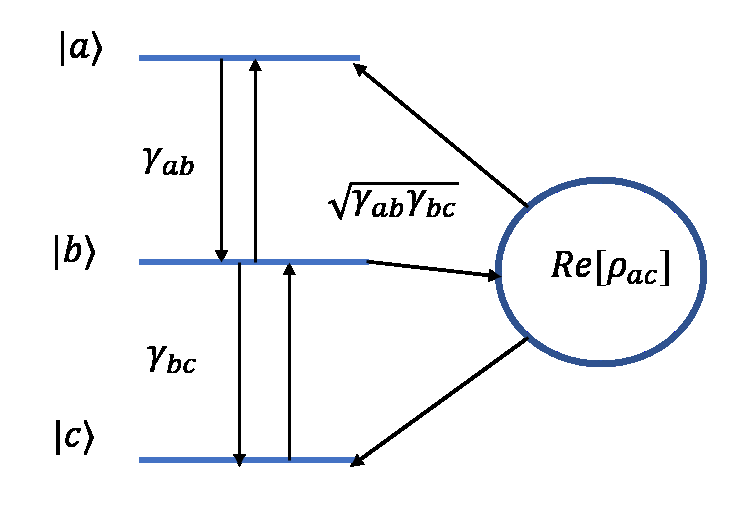
\includegraphics[width=1\columnwidth]{atom_fig3.eps}
\caption{(a) The steady state population distribution for different $\mu_{ab}$ and$\mu_{bc}$. The squeezing parameter $r=1$. (b) The steady state population distribution for non-ideal squeezed vacuum which is characterized by the ratio of $M$ and $\sqrt{N(N+1)}$. (c) The allowed population flow in the squeezed vacuum. The squeezing parameter $r=1$, and $\gamma_{ab}=\frac{1}{4}\gamma_{bc}$.}
\label{2}
\end{figure*}
%\begin{equation}
%\label{eq4}
%\begin{split}
%\frac{d\rho^{S}}{dt}=&\sum_{i\ne j}\frac{\gamma}{2}[-\rho(\cosh rS_{i}^{\dagger}+\sinh rS_{j})(\cosh rS_{i}+\sinh rS_{j}^{\dagger})\\
%&-(\cosh rS_{i}^{\dagger}+\sinh rS_{j})(\cosh rS_{i}+\sinh rS_{j}^{\dagger})\rho\\
%&+2(\cosh rS_{i}+\sinh rS_{j}^{\dagger})\rho(\cosh rS_{i}^{\dagger}+\sinh rS_{j})]
%\end{split}
%\end{equation}

\section{steady state of multiple atoms}
In the last section, we demonstrate that a single atom can achieve steady state population inversion in the squeezed vacuum reservoir. However, with Eq.\eqref{eq2}, this result can not be generated to the multi-atom case since $\gamma'_{ii}=\sqrt{\gamma_{i}\gamma_{i}}\cos[2k_{0z}r_{i}]$. The squeezing term in Eq.\eqref{eq1} vanishes for atoms located around $r_i=\frac{\pi}{4k_{0z}}+\frac{n\pi}{2k_{0z}}$. Thus, for a group of randomly located atoms, if we want to achieve steady state population inversion in the squeezed vacuum, we need to modify our scheme. Here we consider the following correlation functions:
\begin{equation}
\label{eq0b}
\begin{split}
& \left\langle a_{\vec{k},s}^{\dagger}a_{\vec{k}',s'}\right\rangle =\sinh^{2}r\delta_{\vec{k}'\vec{k}}\delta_{ss'} \\
& \left\langle a_{\vec{k},s}a_{\vec{k}',s'}^{\dagger}\right\rangle =\cosh^{2}r\delta_{\vec{k}'\vec{k}}\delta_{ss'}\\
& \left\langle a_{\vec{k},s}^{\dagger}a_{\vec{k}',s'}^{\dagger}\right\rangle =-e^{-i\theta}\cosh(r)\sinh(r)\delta_{\vec{k}',-(2\vec{k}_{0}-\vec{k})}\delta_{ss'}\\
&\left\langle a_{\vec{k},s}a_{\vec{k}',s'}\right\rangle =-e^{i\theta}\cosh(r)\sinh(r)\delta_{\vec{k}',-(2\vec{k}_{0}-\vec{k})}\delta_{ss'}
\end{split}
\end{equation}
which indicates that photons are entangled with those from the opposite direction, then the coefficients in the the master equation Eq.\eqref{eq1} becomes 
\begin{equation}
\label{eq2b}
\begin{split}
& \gamma_{ij}=\sqrt{\gamma_{i}\gamma_{j}}\cos(k_{0z}r_{ij}) \\
& \Lambda_{ij}=\frac{\sqrt{\gamma_{i}\gamma_{j}}}{2}\sin(k_{0z}r_{ij})\\
& \gamma'_{ij}=\sqrt{\gamma_{i}\gamma_{j}}\cos[k_{0z}(r_{ij})]
\end{split}
\end{equation}
which is exactly the traditionally studied master equation\cite{tanas2004stationary} by Ficek. However, they didn't consider the effect of squeezing source, so here we give a detailed derivation on getting Eq. \eqref{eq2b} in Appendix B, where the effect of squeezing source is included. With this new master equation, a single atom can reach population inversion anywhere in the waveguide, as discussed in the Sec. III. When there are multiple atoms in the waveguide, where dipole-dipole interaction needs to be considered, the population inversion still holds true. This is because transition $|a\rangle\leftrightarrow|c\rangle$ is forbidden which results in the fact that dipole-dipole interaction doesn't introduce any extra terms with $\rho_{ac}$. This can be illustrated by looking at the diagonal terms of the first atom in Eq. \eqref{eq1}. Since the general equation is too complicated to analyze, here we just consider a special case where two atoms are located in the waveguide at $r_1=0$ and $r_2=\lambda_{0z}$ respectively, and $\gamma_1=\gamma_2=\gamma$. We also use the rotating wave approximation where oscillating terms are dropped. Then we have the equations for the diagonal terms of the first atom:
\begin{widetext}
\begin{subequations}
\begin{align}
\dot{\rho}_{a_{1},a_{1}}/\gamma=&-ch^{2}\rho_{a_{1},a_{1}}+sh{}^{2}\rho_{b_{1},b_{1}}-\frac{1}{2}chsh(\rho_{a_{1},c_{1}}+\rho_{c_{1},a_{1}})-\frac{1}{2}(\rho_{a_{1}b_{2},b_{1}a_{2}}+\rho_{b_{1}a_{2},a_{1}b_{2}})\label{5a} \\
\dot{\rho}_{b_{1},b_{1}}/\gamma=&(ch^{2}\rho_{a_{1},a_{1}}-sh^{2}\rho_{b_{1},b_{1}})+(sh^{2}\rho_{c_{1},c_{1}}-ch^{2}\rho_{b_{1},b_{1}})+chsh(\rho_{a_{1},c_{1}}+\rho_{c_{1},a_{1}})\nonumber\\
&+\frac{1}{2}(\rho_{a_{1}b_{2},b_{1}a_{2}}+\rho_{b_{1}a_{2},a_{1}b_{2}}-\rho_{b_{1}c_{2},c_{1}b_{2}}-\rho_{c_{1}b_{2},b_{1}c_{2}}) \label{5b}\\
\dot{\rho}_{c_{1},c_{1}}/\gamma=&ch^{2}\rho_{b_{1},b_{1}}-sh^{2}\rho_{c_{1},c_{1}}-\frac{1}{2}chsh(\rho_{a_{1},c_{1}}+\rho_{c_{1},a_{1}})+\frac{1}{2}(\rho_{b_{1}c_{2},c_{1}b_{2}}+\rho_{c_{1}b_{2},b_{1}c_{2}}) \label{5c}
\end{align}
\end{subequations}
\end{widetext}
where notations like $\rho_{a_1, a_1}$ means partial trace of the second atom is taken, i.e., $\rho_{a_1, a_1}=\sum_{i_2=a,b,c}\rho_{a_1i_2, a_1i_2}$, and $\rho_{a_1b_2, b_1a_2}=\langle a_1b_2|\rho|b_1a_2\rangle$. We notice that only the last terms in Eq.\eqref{5a}-\eqref{5c} are the extra terms introduced by the dipole-dipole interaction, and the key role in population inversion $\rho_{ac}$ is not involved in them. Thus, the direct product of each atom's steady state in the single atom case $\frac{sh}{\sqrt{sh^{2}+ch^{2}}}|a\rangle-\frac{ch}{\sqrt{sh^{2}+ch^{2}}}|c\rangle$ is also the solution to Eq.\eqref{5a}-\eqref{5c}. Figure 3(a)(b) shows the steady state population distribution for different decay rate $\gamma_{ab}, \gamma_{bc}$, and for different atomic separation $r_{12}$. We can see that the dipole dipole interaction doesn't play a vital role in the population inversion. Thus, population inversion of a group of atoms can be achieved.

\begin{figure*}
\includegraphics[width=1\columnwidth]{fig3a.eps}
\includegraphics[width=1\columnwidth]{fig3b.eps}
\caption{(a) The steady state population distribution for different $\mu_{ab}$ and$\mu_{bc}$. Three atoms located at $r_1=0, r_2=\lambda_{0z}, r_3=2\lambda_{0z}$ are considered with the squeezing parameter $r=1$. (b) The steady state population distribution as a function of atomic separation for two atoms. The squeezing parameter $r=1$ and $\gamma_{ab}=\frac{1}{4}\gamma_{bc}$.}
\label{2}
\end{figure*}

\section{SUMMARY}
We study the $\Xi$-type atoms coupled to the broadband squeezed vacuum reservoir in a quasi-one-dimensional waveguide, with the overall transition frequency $\omega_{ac}=2\omega_0$. The atoms will evolve into a steady state where most atoms are in the excited state and almost no atoms are in the intemediate state. We also study how the non-perfect squeezing will influence our result. Our main conclusions still hold true when dipole-dipole interaction is considered.

\begin{widetext}
\appendix
\section{DERIVATION OF EQ.\eqref{eq1} }
Here we will show how to derive the master equation Eq. \eqref{eq1}. The interaction Hamiltonian is:
\begin{equation}
\label{eqa0}\tag{A1}
V(t)=-i\hbar \sum_{\vec{k}s}[D(t)a_{\vec{k}s}(t)-D^{+}(t)a^{\dagger}_{\vec{k}s}(t)],
\end{equation}
where
\begin{equation}
\label{eqa1}\tag{A2}
\begin{gathered}
D(t)=\underset{l,i}{\sum}[\vec{\mu}_{l,i}\cdot\vec{u}_{\vec{k},s}(r_{l,i})S_{l,i}^{\dagger}(t)+\vec{\mu}_{l,i}^{*}\cdot\vec{u}_{\vec{k},s}(r_{l,i})S_{l,i}^{-}(t)]
 \end{gathered}
\end{equation}
The reduced master equation of atoms in the reservoir is:
\begin{equation}
\label{eqa2}\tag{A3}
\begin{split}
\frac{d\rho^{S}}{dt}=&-\frac{1}{\hbar^{2}}\int_{0}^{t}d\tau Tr_{F}\{[V(t),[V(t-\tau),\rho^{S}(t-\tau)\rho^{F}\}\\
=&-\frac{1}{\hbar^{2}}\int_{0}^{t}d\tau Tr_{F}\{V(t)V(t-\tau)\rho^{S}(t-\tau)\rho^{F}+\rho^{S}(t-\tau)\rho^{F}V(t-\tau)V(t)\\
&-V(t)\rho^{S}(t-\tau)\rho^{F}V(t-\tau)-V(t-\tau)\rho^{S}(t-\tau)\rho^{F}V(t)\}
\end{split}
\end{equation} 
Here we just show how to deal with the first term in Eq.\eqref{eqa2}, the remaining terms can be calculated in the same way. For the first term, we have
\begin{equation}
\label{eqa3}\tag{A4}
\begin{split}
&-\frac{1}{\hbar^{2}}\int_{0}^{t}d\tau Tr_{F}\{V(t)V(t-\tau)\rho^{S}(t-\tau)\rho^{F}\}\\
=&\int_{0}^{t}d\tau\underset{\vec{k}s,\vec{k}'s'}{\sum}\{D(t)D(t-\tau)Tr_{F}[\rho^{F}a_{ks}(t)a_{k's'}(t-\tau)]-D(t)D^{+}(t-\tau)Tr_{F}[\rho^{F}a_{ks}(t)a^{\dagger}_{k's'}(t-\tau)]\\
&-D^{+}(t)D(t-\tau)Tr_{F}[\rho^{F}a^{\dagger}_{ks}(t)a_{k's'}(t-\tau)]+D^{+}(t)D^{+}(t-\tau)Tr_{F}[\rho^{F}a^{\dagger}_{ks}(t)a^{\dagger}_{k's'}(t-\tau)]\}\rho^{S}(t-\tau)\}.
\end{split}
\end{equation}
Under the rotating wave approximation(RWA), we have
\begin{equation}
\label{eqa4}\tag{A5}
\begin{split}
&-\frac{1}{\hbar^{2}}\int_{0}^{t}d\tau Tr_{F}\{V(t)V(t-\tau)\rho^{S}(t-\tau)\rho^{F}\}\\
=&\sum_{ijlm}\underset{\vec{k}s,\vec{k'}s'}{\sum}\int_{0}^{t}d\tau\{\vec{\mu}{}_{l,i}\cdot\vec{u}_{\vec{k}s}(r_{l,i})S_{l,i}^{+}e^{i\omega_{i}t}\vec{\mu}_{m,j}\cdot\vec{u}_{\vec{k}'s'}(r_{m,j})S_{m,j}^{+}e^{i\omega_{j}(t-\tau)}e^{-i(\omega_{\vec{k}s}+\omega_{\vec{k}'s'})t+i\omega_{\vec{k}'s'}\tau}[-\sinh(r)\cosh(r)\delta_{\vec{k}',2\vec{k}_{0}-\vec{k}}\delta_{ss'}]\\
&-\vec{\mu}_{l,i}\cdot\vec{u}_{\vec{k}s}(r_{l,i})S_{l,i}^{+}e^{i\omega_{i}t}\vec{\mu}_{m,j}^{*}\cdot\vec{u}_{\vec{k}'s'}^{*}(r_{m,j})S_{m,j}^{-}e^{-i\omega_{j}(t-\tau)}e^{-i\omega_{\vec{k}'s'}\tau}\cosh^{2}r\delta_{\vec{k}\vec{k}'}\delta_{ss'}\\
&-\vec{\mu}_{l,i}^{*}\cdot\vec{u}_{\vec{k}s}(r_{l,i})S_{l,i}^{-}e^{-i\omega_{i}t}\vec{\mu}_{m,j}\cdot\vec{u}_{\vec{k}'s'}^{*}(r_{m,j})S_{m,j}^{+}e^{i\omega_{j}(t-\tau)}e^{-i\omega_{\vec{k}'s'}\tau}\cosh^{2}r\delta_{\vec{k}\vec{k}'}\delta_{ss'}\\
&-\vec{\mu}_{l,i}^{*}\cdot\vec{u}_{\vec{k}s}^{*}(r_{l,i})S_{l,i}^{-}e^{-i\omega_{i}t}\vec{\mu}_{m,j}\cdot\vec{u}_{\vec{k}'s'}(r_{m,j})S_{m,j}^{+}e^{i\omega_{j}(t-\tau)}e^{i\omega_{\vec{k}'s'}\tau}\sinh^{2}r\delta_{\vec{k}\vec{k}'}\delta_{ss'}\\
&-\vec{\mu}_{l,i}\cdot\vec{u}_{\vec{k}s}^{*}(r_{l,i})S_{l,i}^{+}e^{i\omega_{i}t}\vec{\mu}_{m,j}^{*}\cdot\vec{u}_{\vec{k}'s'}(r_{m,j})S_{m,j}^{-}e^{-i\omega_{j}(t-\tau)}e^{i\omega_{\vec{k}'s'}\tau}\sinh^{2}r\delta_{\vec{k}\vec{k}'}\delta_{ss'}\\
&+\vec{\mu}_{l,i}^{*}\cdot\vec{u}_{\vec{k}s}^{*}(r_{l,i})S_{l,i}^{-}e^{-i\omega_{i}t}\vec{\mu}_{m,j}^{*}\cdot\vec{u}_{\vec{k}'s'}^{*}(r_{m,j})S_{m,j}^{-}e^{-i\omega_{j}(t-\tau)}e^{i(\omega_{\vec{k}s}+\omega_{\vec{k}'s'})t-i\omega_{\vec{k}'s'}\tau}[-\sinh(r)\cosh(r)\delta_{\vec{k}',2\vec{k}_{0}-\vec{k}}\delta_{ss'}]\}\rho^{S}(t-\tau)
\end{split}
\end{equation}
where $l,m$ are used for labeling different atoms, and $i,j$ are used for transitions within an atom. Here we just calculate the first and second term to show how to get the master equation Eq.\eqref{eq1}. Since all atoms are identical, $\omega_{l,i}=\omega_{i}$, $|\vec\mu_{l,i}|=|\vec\mu_i|$, and $r_{l,i}=r_{l}$ can be used to simplify Eq.\eqref{eqa4}. For the second term(thermal term), we have
\begin{equation}
\label{eqc2}\tag{A6}
\begin{split}
&-\underset{k_{z}}{\sum}\int_{0}^{t}d\tau\vec{\mu}_{l,i}\cdot\vec{u}_{\vec{k}s}(r_{l})S_{l,i}^{+}e^{i\omega_{i}t}\vec{\mu}_{m,j}^{*}\cdot\vec{u}_{\vec{k}'s'}^{*}(r_{m})S_{m,j}^{-}e^{-i\omega_{j}(t-\tau)}e^{-i\omega_{\vec{k}'s'}\tau}\cosh^{2}r\rho^{S}(t-\tau)\delta_{\vec{k}\vec{k}'}\delta_{ss'}\\
=&-\frac{L}{2\pi}e^{i(\omega_{i}-\omega_{j})t}\int_{-\infty}^{\infty}dk_{z}\int_{0}^{t}d\tau e^{i\omega_{j}\tau}e^{-i\omega_{k_{z}}\tau}\frac{\omega_{k}\mu_{i}\mu_{j}}{\epsilon_{0}LS\hbar}e^{ik_{z}(r_{l}-r_{m})}\cosh^{2}rS_{l,i}^{+}S_{m,j}^{-}\rho^{S}(t-\tau)\\
\approx&-\frac{L}{2\pi}e^{i(\omega_{i}-\omega_{j})t}\int_{0}^{\infty}dk_{z}\int_{0}^{t}d\tau e^{i\omega_{j}\tau}e^{-i[\omega_{j}+c^{2}k_{jz}(k_{z}-k_{jz})/\omega_{j}]\tau}\frac{\omega_{k}\mu_{i}\mu_{j}}{\epsilon_{0}LS\hbar}[e^{ik_{z}(r_{l}-r_{m})}+e^{-ik_{z}(r_{l}-r_{m})}]\cosh^{2}rS_{l,i}^{+}S_{m,j}^{-}\rho^{S}(t-\tau)\\
\approx&-\frac{L}{2\pi}e^{i(\omega_{i}-\omega_{j})t}\int_{-k_{0z}}^{\infty}d\delta k_{z}\int_{0}^{t}d\tau e^{-i\tau c^{2}k_{jz}\delta k_{z}/\omega_{j}}\frac{\omega_{k}\mu_{i}\mu_{j}}{\epsilon_{0}LS\hbar}[e^{i(k_{jz}+\delta k_{z})(r_{l}-r_{m})}+e^{-i(k_{jz}+\delta k_{z})(r_{l}-r_{m})}]\cosh^{2}rS_{l,i}^{+}S_{m,j}^{-}\rho^{S}(t-\tau)\\
\approx&-\frac{L}{2\pi}e^{i(\omega_{i}-\omega_{j})t}\int_{-\infty}^{\infty}d\delta k_{z}\int_{0}^{t}d\tau e^{-i(c^{2}k_{jz}\delta k_{z}/\omega_{j})\tau}\frac{\omega_{k}\mu_{i}\mu_{j}}{\epsilon_{0}LS\hbar}[e^{i(k_{jz}+\delta k_{z})(r_{l}-r_{m})}+e^{-i(k_{jz}+\delta k_{z})(r_{l}-r_{m})}]\cosh^{2}rS_{l,i}^{+}S_{m,j}^{-}\rho^{S}(t-\tau)\\
\approx&-\frac{L}{2\pi}e^{i(\omega_{i}-\omega_{j})t}\int_{0}^{t}d\tau\frac{\omega_{j}\mu_{i}\mu_{j}}{\epsilon_{0}LS\hbar}2\pi[e^{ik_{jz}(r_{l}-r_{m})}\delta((r_{l}-r_{m})-\frac{c^{2}k_{jz}}{\omega_{0}}\tau)+e^{-ik_{jz}(r_{l}-r_{m})}\delta((r_{l}-r_{m})+\frac{c^{2}k_{jz}}{\omega_{0}}\tau)]\cosh^{2}rS_{l,i}^{+}S_{m,j}^{-}\rho^{S}(t-\tau)\\
\approx&-\frac{L}{2\pi}e^{ik_{jz}r_{lm}}\frac{\omega_{j}\mu_{i}\mu_{j}}{\epsilon_{0}LS\hbar}2\pi\frac{\omega_{j}}{c^{2}k_{0z}}\cosh^{2}rS_{l,i}^{+}S_{m,j}^{-}\rho^{S}(t)e^{i(\omega_{i}-\omega_{j})t}\\
\approx&-[\frac{\sqrt{\gamma_{i}\gamma_{j}}}{2}\cos(k_{0z}r_{lm})+i\frac{\sqrt{\gamma_{i}\gamma_{j}}}{2}sin(k_{0z}r_{lm})]\cosh^{2}rS_{l,i}^{+}S_{m,j}^{-}\rho^{S}(t)e^{i(\omega_{i}-\omega_{j})t}\\
\end{split}
\end{equation}
where emitter separation $r_{lm}=|r_{l}-r_{m}|$, collective decay rate $\gamma_{i}=2\mu_{i}^{2}\omega_{i}^{2}/\hbar\epsilon_{0}Sc^{2}k_{iz}$, and collective energy shift $\Lambda_{ij}=\sqrt{\gamma_{i}\gamma_{j}}\sin(k_{0z}r_{ij})/2$.
In the third line we expand $\omega_{k}=c\sqrt{(\frac{\pi}{a})^{2}+(k_{z})^{2}}$ around $k_{z}=k_{0z}$ since resonant modes provide dominant contributions. In the fifth line we extend the integration $\int_{-k_{jz}}^{\infty}dk_{z}\rightarrow\int_{-\infty}^{\infty}dk_{z}$ because the main contribution comes from the components around $\delta k_{z}=0$. In the next line, Weisskopf-Wigner approximation is used. Since index $i$ and $j$ are always associated with index $l$ and $m$ respectively, we can combine $l,i$ as $i$, and $m,j$ as $j$ for simplicity. Thus, we have obtained $\gamma_{ij}$ and $\Lambda_{ij}$ as is shown in Eq.\eqref{eq2}. 

Next we need to calculate the first term (squeezing term) in Eq.\eqref{eqa4}:
\begin{equation}
\label{eqb8}\tag{A7}
\begin{split}
& e^{i(\omega_{i}+\omega_{j}-2\omega_{0})t}\underset{k_{z}}{\sum}\int_{0}^{t}d\tau\{\vec{\mu}{}_{l,i}\cdot\vec{u}_{2\vec{k}_{0}-\vec{k}}(r_{l})S_{l,i}^{+}\vec{\mu}_{m,j}\cdot\vec{u}_{\vec{k}}(r_{m})S_{m,j}^{+}e^{i(\omega_{\vec{k}}-\omega_{j})\tau}[-\sinh(r)\cosh(r)]\rho^{S}(t-\tau)\\
=&-\frac{L}{2\pi}e^{i(\omega_{i}+\omega_{j}-2\omega_{0})t}\int_{0}^{2k_{0z}}dk_{z}\int_{0}^{t}d\tau e^{i(\omega_{k_{z}}-\omega_{j})\tau}e^{i(2k_{jz}-k_{z})(r_{l}-o_{1})}e^{ik_{z}(r_{m}-o_{1})}\frac{\sqrt{\omega_{k_{z}}\omega_{2k_{0z}-k_{z}}}\mu_{i}\mu_{j}}{\epsilon_{0}LS\hbar}\sinh(r)\cosh(r)S_{l,i}^{+}S_{m,j}^{+}\rho^{S}(t-\tau)\\ 
&-\frac{L}{2\pi}e^{i(\omega_{i}+\omega_{j}-2\omega_{0})t}\int_{-2k_{0z}}^{0}dk_{z}\int_{0}^{t}d\tau e^{i(\omega_{k_{z}}-\omega_{j})\tau}e^{i(-2k_{jz}-k_{z})(r_{l}-o_{2})}e^{ik_{z}(r_{m}-o_{2})}\frac{\sqrt{\omega_{k_{z}}\omega_{-2k_{0z}-k_{z}}}\mu_{i}\mu_{j}}{\epsilon_{0}LS\hbar}\sinh(r)\cosh(r)S_{l,i}^{+}S_{m,j}^{+}\rho^{S}(t-\tau)
\end{split}
\end{equation}
Putting aside the overall factor $e^{i(\omega_i+\omega_j-2\omega_0)t}$, for $r_l=r_j$, Eq.\eqref{eqb8} reduces to 
\begin{equation}
\label{eqb9}\tag{A8}
\begin{split}
&\underset{k_{z}}{\sum}\int_{0}^{t}d\tau\{\vec{\mu}{}_{l,i}\cdot\vec{u}_{2\vec{k}_{0}-\vec{k}}(r_{l})S_{l,i}^{+}\vec{\mu}_{l,j}\cdot\vec{u}_{\vec{k}}(r_{l})S_{l,j}^{+}e^{i(\omega_{\vec{k}}-\omega_{j})\tau}[-\sinh(r)\cosh(r)]\rho^{S}(t-\tau)\\
=&-\frac{L}{2\pi}\int_{0}^{2k_{0z}}dk_{z}\int_{0}^{t}d\tau e^{i\frac{c^{2}k_{jz}}{_{\omega_{j}}}(k_{z}-k_{jz})\tau}e^{i2k_{0z}(r_{l}-o_{1})}\frac{\sqrt{\omega_{k_{z}}\omega_{2k_{0z}-k_{z}}}\mu_{i}\mu_{j}}{\epsilon_{0}LS\hbar}\sinh(r)\cosh(r)S_{l,i}^{+}S_{l,j}^{+}\rho^{S}(t-\tau)\\
&-\frac{L}{2\pi}\int_{-2k_{0z}}^{0}dk_{z}\int_{0}^{t}d\tau e^{i\frac{c^{2}k_{jz}}{_{\omega_{j}}}(k_{z}-k_{jz})\tau}e^{-i2k_{0z}(r_{l}-o_{2})}\frac{\sqrt{\omega_{k_{z}}\omega_{-2k_{0z}-k_{z}}}\mu_{i}\mu_{j}}{\epsilon_{0}LS\hbar}\sinh(r)\cosh(r)S_{l,i}^{+}S_{l,j}^{+}\rho^{S}(t-\tau)\\
=&-\frac{L}{2\pi}[e^{i2k_{0z}(r_{l}-o_{1})}+e^{-i2k_{0z}(r_{l}-o_{2})}]\frac{\sqrt{\omega_{i}\omega_{j}}\mu_{i}\mu_{j}}{\epsilon_{0}LS\hbar}\int_{0}^{t}d\tau2\pi\delta(\frac{c^{2}k_{jz}}{\omega_{j}}\tau)\sinh(r)\cosh(r)S_{l,i}^{+}S_{l,j}^{+}\rho^{S}(t-\tau)\\
=&-e^{i2k_{jz}R}\frac{\omega_{0}^{2}\mu_{i}\mu_{j}}{\epsilon_{0}\hbar Sc^{2}k_{0z}}\cos(2k_{0z}r_{l})\sinh(r)\cosh(r)S_{l,i}^{+}S_{l,j}^{+}\rho^{S}(t)\\
=&-e^{i2k_{0z}R}\frac{\sqrt{\gamma_{i}\gamma_{j}}}{2}\cos(2k_{0z}r_{l})\sinh(r)\cosh(r)S_{l,i}^{+}S_{l,j}^{+}\rho^{S}(t)
\end{split}
\end{equation}
where we have used the fact that the origin of coordinate system is at equal distant from two sources(i.e., $o_2=-o_1=R$) in the second last line. Incorporating index $l$ into $i$, we have $\gamma'_{ij}=\sqrt{\gamma_{i}\gamma_{j}}\cos(2k_{0z}r_{i})$. For $r_i\neq r_j$, Eq. \eqref{eqb8} reduces to
\begin{equation}
\label{eqb10}\tag{A9}
\begin{split}
&\underset{k_{z}}{\sum}\int_{0}^{t}d\tau\{\vec{\mu}{}_{l,i}\cdot\vec{u}_{2\vec{k}_{0}-\vec{k}}(r_{l})S_{l,i}^{+}\vec{\mu}_{m,j}\cdot\vec{u}_{\vec{k}}(r_{m})S_{m,j}^{+}e^{i(\omega_{\vec{k}}-\omega_{j})\tau}[-\sinh(r)\cosh(r)]\rho^{S}(t-\tau)\\
=&-\frac{L}{2\pi}\int_{0}^{2k_{0z}}dk_{z}\int_{0}^{t}d\tau e^{i\frac{c^{2}k_{jz}}{_{\omega_{j}}}(k_{z}-k_{jz})\tau}e^{i2k_{0z}(r_{c}-o_{1})}e^{-i(k_{z}-k_{0z})(r_{l}-r_{m})}\frac{\sqrt{\omega_{k_{z}}\omega_{2k_{0z}-k_{z}}}\mu_{i}\mu_{j}}{\epsilon_{0}LS\hbar}\sinh(r)\cosh(r)S_{l,i}^{+}S_{m,j}^{+}\rho^{S}(t-\tau) \\
& -\frac{L}{2\pi}\int_{-2k_{0z}}^{0}dk_{z}\int_{0}^{t}d\tau e^{i\frac{c^{2}k_{jz}}{_{\omega_{j}}}(-k_{z}-k_{jz})\tau}e^{-i2k_{0z}(r_{c}-o_{2})}e^{-i(k_{z}+k_{0z})(r_{l}-r_{m})}\frac{\sqrt{\omega_{k_{z}}\omega_{-2k_{0z}-k_{z}}}\mu_{i}\mu_{j}}{\epsilon_{0}LS\hbar}\sinh(r)\cosh(r)S_{l,i}^{+}S_{m,j}^{+}\rho^{S}(t-\tau)\\
=&-\frac{L}{2\pi}e^{i2k_{0z}(r_{c}-o_{1})}\frac{\sqrt{\omega_{i}\omega_{j}}\mu_{i}\mu_{j}}{\epsilon_{0}LS\hbar}\int_{-\infty}^{\infty}dk_{z}\int_{0}^{t}d\tau e^{i\frac{c^{2}k_{jz}}{_{\omega_{j}}}(k_{z}-k_{jz})\tau}e^{-i(k_{z}-k_{0z})(r_{l}-r_{m})}\sinh(r)\cosh(r)S_{l,i}^{+}S_{m,j}^{+}\rho^{S}(t-\tau)\\
&-\frac{L}{2\pi}e^{-i2k_{0z}(r_{c}-o_{2})}\frac{\sqrt{\omega_{i}\omega_{j}}\mu_{i}\mu_{j}}{\epsilon_{0}LS\hbar}\int_{-\infty}^{\infty}dk_{z}\int_{0}^{t}d\tau e^{i\frac{c^{2}k_{jz}}{_{\omega_{j}}}(k_{z}-k_{jz})\tau}e^{i(k_{z}-k_{0z})(r_{l}-r_{m})}\sinh(r)\cosh(r)S_{l,i}^{+}S_{m,j}^{+}\rho^{S}(t-\tau) \\
\approx&-\frac{L}{2\pi}e^{i2k_{0z}R}\frac{\omega_{0}^{2}\mu_{i}\mu_{j}}{\epsilon_{0}LS\hbar}\int_{0}^{t}d\tau2\pi[e^{i2k_{0z}r_{c}}\delta(r_{l}-r_{m}-\frac{c^{2}k_{0z}}{_{\omega_{0}}}\tau)+e^{-i2k_{0z}r_{c}}\delta(r_{l}-r_{m}+\frac{c^{2}k_{0z}}{_{\omega_{0}}}\tau)]\sinh(r)\cosh(r)S_{l,i}^{+}S_{m,j}^{+}\rho^{S}(t-\tau) \\
\approx&-e^{i2k_{0z}R}\frac{\omega_{0}^{2}\mu_{i}\mu_{j}}{\epsilon_{0}\hbar Sc^{2}k_{0z}}e^{i2k_{0z}r_{c}sgn(r_{l}-r_{m})}S_{l,i}^{+}S_{m,j}^{+}\rho^{S}(t)\rightarrow-\frac{\sqrt{\gamma_{i}\gamma_{j}}}{2}e^{i2k_{0z}R}\cos(k_{0z}(r_{l}+r_{m}))S_{l,i}^{+}S_{m,j}^{+}\rho^{S}(t)\\
\end{split}
\end{equation}
where $sgn(r_{l}-r_{m})$ is the sign function. The last arrow is because we need to sum over $i,j$, so the imaginary part of $e^{i2k_{0z}r_{c}sgn(i-j)}$ vanishes, so the neat result is that $\gamma'_{ij}=e^{i2k_{0z}R}\sqrt{\gamma_{i}\gamma_{j}}\cos(k_{0z}(r_{i}+r_{j}))$ after combining index $l,i$ and $m,j$ as $i$ and $j$. As for $S_{i}^{+}\rho^{S}(t)S_{j}^{+}$ terms, the combination of the last two terms in Eq.\eqref{eqa2} will make the imaginary part of $e^{i2k_{0z}r_{c}sgn(r_{l}-r_{m})}$ vanish. Thus, we have $\gamma'_{ij}=e^{i2k_{0z}R}\sqrt{\gamma_{i}\gamma_{j}}\cos(k_{0z}(r_i+r_j))$ in Eq.\eqref{eq2}. 

\section{DERIVATION OF coefficients EQ.\eqref{eq2b} }
Here we will show how to derive the master equation with coefficients Eq.\eqref{eq2b} from the correlation function Eq. \eqref{eq0b}. Since the only difference is the squeezing terms $\left\langle a_{\vec{k},s}^{\dagger}a_{\vec{k}',s'}^{\dagger}\right\rangle$, $\left\langle a_{\vec{k},s}a_{\vec{k}',s'}\right\rangle $, we will just start from Eq. \eqref{eqb8}. Apart from the factor $e^{i(\omega_i+\omega_j-2\omega_0)t}$, When $r_i\ne r_j$, Eq. \eqref{eqb8} becomes:

\begin{equation}
\label{eqb1}\tag{B1}
\begin{split}
&\underset{k_{z}}{\sum}\int_{0}^{t}d\tau\{\vec{\mu}{}_{l,i}\cdot\vec{u}_{-2\vec{k}_{0}+\vec{k}}(r_{l})S_{l,i}^{+}\vec{\mu}_{m,j}\cdot\vec{u}_{\vec{k}}(r_{m})S_{m,j}^{+}e^{i(\omega_{\vec{k}}-\omega_{0})\tau}[-\sinh(r)\cosh(r)]\rho^{S}(t-\tau)\\
\approx&-\frac{L}{2\pi}\int_{0}^{2k_{0}}dk\int_{0}^{t}d\tau e^{i\frac{c^{2}k_{0}}{_{\omega_{0}}}(k-k_{0})\tau}e^{-i(2k_{0}-k)(r_{l}-o_{2})+ik(r_{m}-o_{1})}\frac{\sqrt{\omega_{k_{z}}\omega_{2k_{0z}-k_{z}}}\mu_{i}\mu_{j}}{\epsilon_{0}LS\hbar}\sinh(r)\cosh(r)S_{l,i}^{+}S_{m,j}^{+}\rho^{S}(t-\tau)\\
&-\frac{L}{2\pi}\int_{-2k_{0}}^{0}dk\int_{0}^{t}d\tau e^{i\frac{c^{2}k_{0}}{_{\omega_{0}}}(-k-k_{0})\tau}e^{i(2k_{0}+k)(r_{l}-o_{2})+ik(r_{m}-o_{1})}\frac{\sqrt{\omega_{k_{z}}\omega_{-2k_{0z}-k_{z}}}\mu_{i}\mu_{j}}{\epsilon_{0}LS\hbar}\sinh(r)\cosh(r)S_{l,i}^{+}S_{m,j}^{+}\rho^{S}(t-\tau)\\
=&-\frac{L}{2\pi}\int_{0}^{2k_{0}}dk\int_{0}^{t}d\tau e^{i\frac{c^{2}k_{0}}{_{\omega_{0}}}(-k_{0})\tau}e^{-i(2k_{0})(r_{l}-o_{2})}e^{ik(\frac{c^{2}k_{0}}{_{\omega_{0}}}\tau+r_{l}-o_{1}+r_{m}-o_{2})}\frac{\sqrt{\omega_{k_{z}}\omega_{2k_{0z}-k_{z}}}\mu_{i}\mu_{j}}{\epsilon_{0}LS\hbar}\sinh(r)\cosh(r)S_{l,i}^{+}S_{m,j}^{+}\rho^{S}(t-\tau)\\
&-\frac{L}{2\pi}\int_{0}^{2k_{0}}dk\int_{0}^{t}d\tau e^{i\frac{c^{2}k_{0}}{_{\omega_{0}}}(-k_{0})\tau}e^{i(2k_{0})(r_{l}-o_{2})}e^{ik(\frac{c^{2}k_{0}}{_{\omega_{0}}}\tau-r_{l}+o_{1}-r_{m}+o_{2})}\frac{\sqrt{\omega_{k_{z}}\omega_{-2k_{0z}-k_{z}}}\mu_{i}\mu_{j}}{\epsilon_{0}LS\hbar}\sinh(r)\cosh(r)S_{l,i}^{+}S_{m,j}^{+}\rho^{S}(t-\tau)\\
\approx&-\frac{L}{2\pi}\int_{0}^{t}d\tau e^{i\frac{c^{2}k_{0}}{_{\omega_{0}}}(-k_{0})\tau}e^{-i(2k_{0})(r_{l})}e^{2ik_{0}o_{2}}2\pi\delta(\frac{c^{2}k_{0}}{_{\omega_{0}}}\tau+2r_{c}-o_{1}-o_{2})\frac{\sqrt{\omega_{i}\omega_{j}}\mu_{i}\mu_{j}}{\epsilon_{0}LS\hbar}\sinh(r)\cosh(r)S_{l,i}^{+}S_{m,j}^{+}\rho^{S}(t-\tau)\\
&-\frac{L}{2\pi}\int_{0}^{t}d\tau e^{i\frac{c^{2}k_{0}}{_{\omega_{0}}}(-k_{0})\tau}e^{i(2k_{0})(r_{l})}e^{-2ik_{0}o_{2}}2\pi\delta(\frac{c^{2}k_{0}}{_{\omega_{0}}}\tau-2r_{c}+o_{1}+o_{2})\frac{\sqrt{\omega_{i}\omega_{j}}\mu_{i}\mu_{j}}{\epsilon_{0}LS\hbar}\sinh(r)\cosh(r)S_{l,i}^{+}S_{m,j}^{+}\rho^{S}(t-\tau)\\
\approx&-\frac{L}{2\pi}e^{i(-k_{0})|2r_{c}-o_{1}-o_{2}|}e^{sgn(r_{c}-o_{1}-o_{2})i(2k_{0})(r_{l})}e^{-2ik_{0}o_{2}}2\pi\frac{\omega_{0}^{2}\mu_{i}\mu_{j}}{\epsilon_{0}LS\hbar c^{2}k_{0z}}\sinh(r)\cosh(r)S_{l,i}^{+}S_{m,j}^{+}\rho^{S}(t)\\
=&-\frac{L}{2\pi}e^{sgn(2r_{c}-o_{1}-o_{2})ik_{0}(r_{l}-r_{m})}e^{ik_{0}(o_{1}-o_{2})}2\pi\frac{\omega_{0}^{2}\mu_{i}\mu_{j}}{\epsilon_{0}LS\hbar c^{2}k_{0z}}\sinh(r)\cosh(r)S_{l,i}^{+}S_{m,j}^{+}\rho^{S}(t)
\end{split}
\end{equation}
Since we need to sum over $l,m,i,j$, the imaginary part of $e^{sgn(2r_{c}-o_{1}-o_{2})ik_{0}(r_{l}-r_{m})}$ gets canceled, which yields $\gamma'_{ij}=\sqrt{\gamma_{i}\gamma_{j}}\cos[k_{0z}(r_{ij})]$. The above calculation is also valid when $r_i=rj$.

\end{widetext}

\bibliography{ref}
%\begin{thebibliography}{99}
%end{thebibliography}
\end{document}